\section{Accumulator concept}
\label{sec:accumulator-approach}



A simple concept, named \textit{accumulator}, has been proposed to improve MPI communication during a Jacobian matrix transfer preserving the current AHLET-NuT architecture and coupling.\\


The concept represents two arrays of length $2L$ where the first one, called \textit{accumulator}, is used for accumulation of Jacobian matrix elements, stored in compressed sparse matrix format, till the critical array length equaled to $L = F \cdot N$, where $N$ is a size of the underlying Jacobian matrix and $F$ is a so-called capacity factor. Once the current array length of \textit{accumulator} exceeds its critical length, the accumulated data are moved to \textit{send buffer} by means of a simple swap of pointers, \textit{ACC\_PTR} and \textit{SEND\_BUFF\_PTR}, see figure \ref{fig:accumulator-concept}. Having swapped the pointers and reset control variables, accumulation procedure can be immediately continued together with an immediate instantiation of the corresponding non-blocking broadcast operation with respect to \textit{send buffer} content.\\


\begin{figure}[htpb]
  \centering
  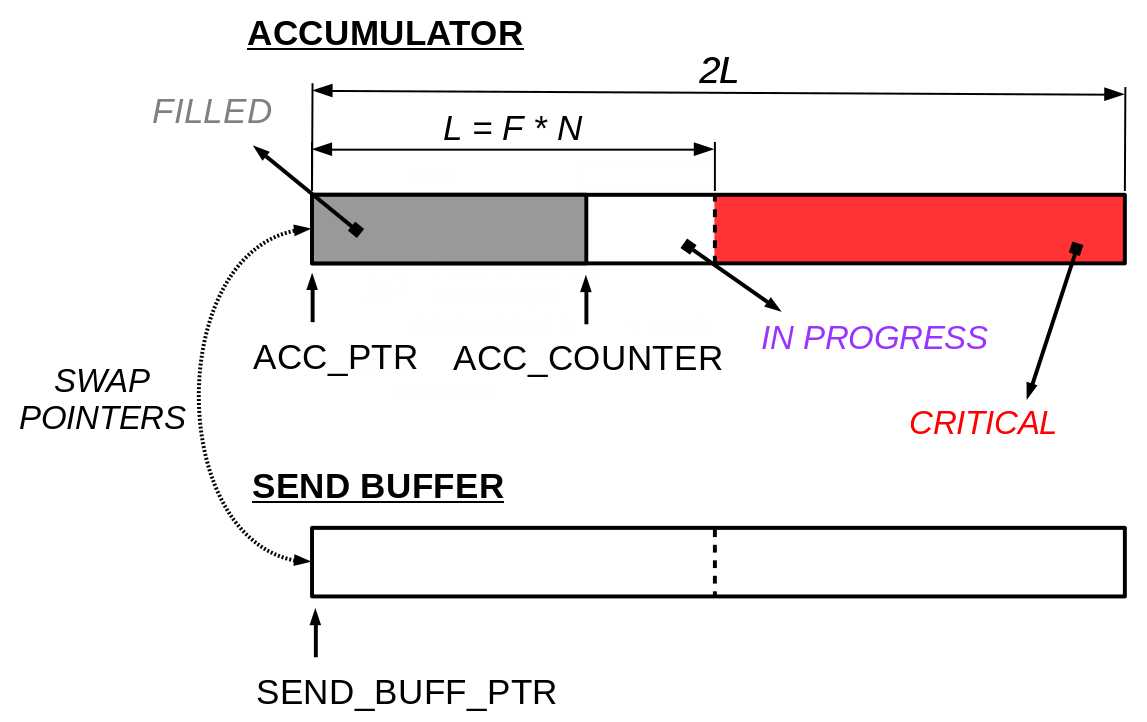
\includegraphics[width=0.8\textwidth]{figures/chapter-3/accumulator-concept.png}
  \caption{Accumulator concept} \label{fig:accumulator-concept}
\end{figure}


The second array part of \textit{accumulator}, also called the critical part, is used for safe placement of data surplus without any extra program checks and manipulations, using an assumption that a column vector cannot exceed the Jacobian matrix size. The assumption is based on long-term and first-hand experience of ATHLET-NuT users. On another hand, the event, described above, triggers a signal for a regular pointer swap and, therefore, the subsequent non-blocking data transfer.\\


The factor $F$, depicted in figure \ref{fig:accumulator-concept}, can be used by the user for two purposes. Mainly, it allows the user to adjust the \textit{send buffer} length $L$ till the point of saturation of physical interconnection bandwidth, see figure \ref{fig:hw1-bandwidth} as an example, and, thus, achieve efficient resource utilization. Secondly, as a result, it reduces the amount of handshakes, the amount of resource acquisition requests, between NuT and clients. The default value of the factor is equal to 1, however, we insistently recommend to increase the value via the corresponding environment variable for small-sized problems and operation of NuT in a multi-client mode.\\


\begin{figure}[htpb]
  \centering
  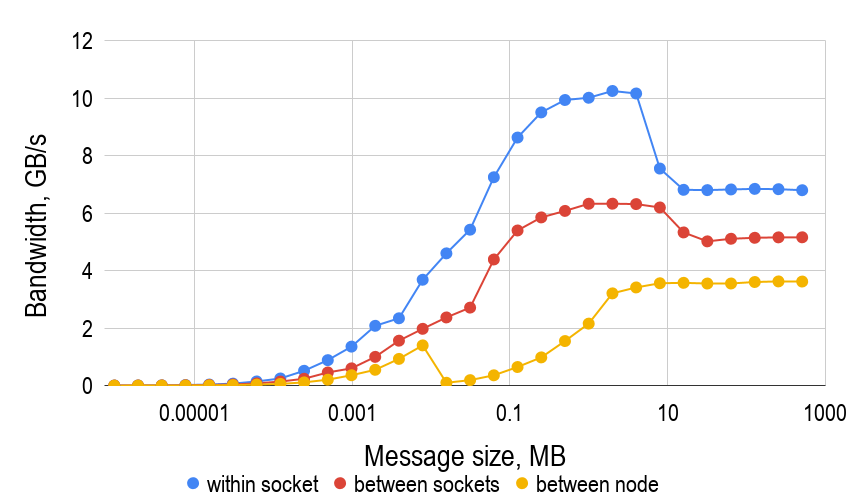
\includegraphics[width=0.8\textwidth]{figures/chapter-3/hw1-bandwidth.png}
  \caption{Technical characteristics of HW1 interconnection} \label{fig:hw1-bandwidth}
\end{figure}



Figure \ref{fig:accumulator-in-action} represents application of the \textit{accumulator} algorithm to the example represented in figure \ref{fig:matrix-column-distribution} with the following parameters: $N = 100$ and $F = 1$. It can be easily observed the algorithm reduces the number of transfers from 28 to 12. Additionally, the average column length, excluding the last one, jumps from 56 to 131. By and large, the algorithm allows to transform the original distribution shape to a more or less rectangular one that, in its turns, allows to transfer the matrix in approximately equal chunks.\\



\figpointer{\ref{fig:accumulator-in-action}}
\begin{figure}[htpb]
\centering
	\begin{tabular}{cc}
		\subfloat[Before]{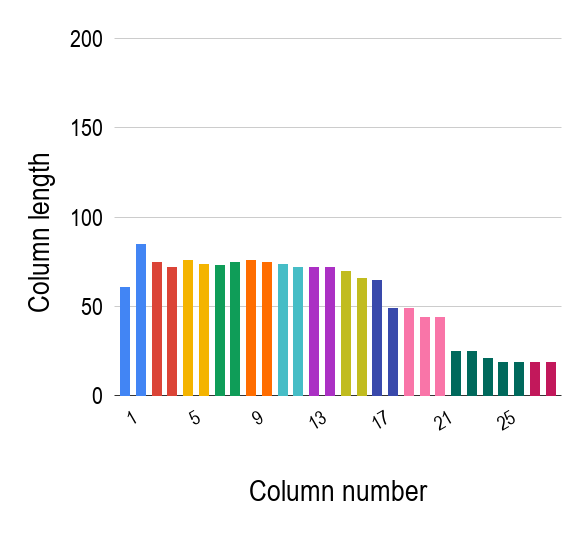
\includegraphics[width=0.48\textwidth]{figures/chapter-3/accumulation-before.png}} &
		\subfloat[After]{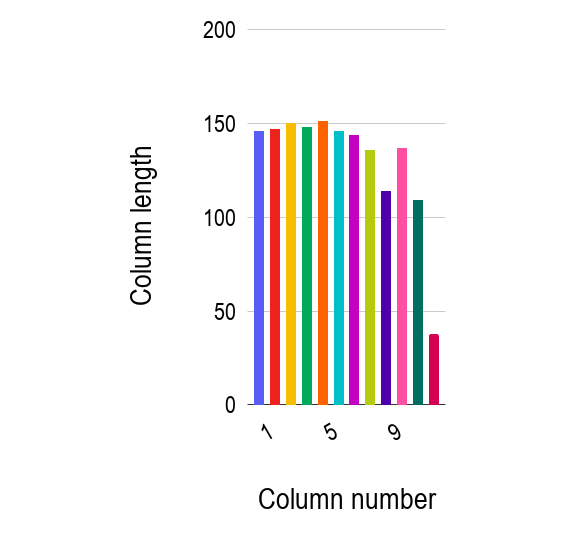
\includegraphics[width=0.48\textwidth]{figures/chapter-3/accumulation-after.png}} \\
	\end{tabular}
	\caption{Application the of \textit{accumulator} concept to the example depicted in figure \ref{fig:matrix-column-distribution}, with $N=100$ and $F=1$}
	\label{fig:accumulator-in-action}
\end{figure}


Before ATHLET can send a request to NuT to start solution of systems \ref{eq:athlet-10} it has to be certain about the entire Jacobian matrix has been transfered to the NuT side. For that reason, the last column transfer is done by means of the corresponding blocking MPI operations. It means ATHLET gets blocked only during the last column transfer and MPI gives the execution control back only when the last piece data has been successfully distributed among NuT processes.\\ 
